%%%%%%%%%%%%%%%%%%%%%%%%%%%%%%%%%%%%%%%%%%%%%%%%%%%%%%
% A Beamer template for University of Wollongong     %
% Based on THU beamer theme                          %
% Author: Qiuyu Lu                                   %
% Date: July 2024                                    %
% LPPL Licensed.                                     %
%%%%%%%%%%%%%%%%%%%%%%%%%%%%%%%%%%%%%%%%%%%%%%%%%%%%%%
% Customized for Sharif University of Technology     %
%%%%%%%%%%%%%%%%%%%%%%%%%%%%%%%%%%%%%%%%%%%%%%%%%%%%%%


\documentclass[serif, aspectratio=169]{beamer}
%\documentclass[serif]{beamer}  % for 4:3 ratio
\usepackage[T1]{fontenc} 
\usepackage{fourier} % see "http://faq.ktug.org/wiki/uploads/MathFonts.pdf" for other options
\usepackage{hyperref}
\usepackage{latexsym,amsmath,xcolor,multicol,booktabs,calligra}
\usepackage{graphicx,pstricks,listings,stackengine}
\usepackage{lipsum}
\usepackage{algorithm, algpseudocode, mathtools, needspace}


\author{Ali Sharifi-Zarchi}
\title{Machine Learning (CE 40717)}
\subtitle{Fall 2024}
\institute{
    CE Department \\
    Sharif University of Technology
}
%\date{\small \today}
% \usepackage{UoWstyle}
\usepackage{SUTstyle}

% defs
\def\cmd#1{\texttt{\color{red}\footnotesize $\backslash$#1}}
\def\env#1{\texttt{\color{blue}\footnotesize #1}}
\definecolor{deepblue}{rgb}{0,0,0.5}
\definecolor{deepred}{RGB}{153,0,0}
\definecolor{deepgreen}{rgb}{0,0.5,0}
\definecolor{halfgray}{gray}{0.55}

\lstset{
    basicstyle=\ttfamily\small,
    keywordstyle=\bfseries\color{deepblue},
    emphstyle=\ttfamily\color{deepred},    % Custom highlighting style
    stringstyle=\color{deepgreen},
    numbers=left,
    numberstyle=\small\color{halfgray},
    rulesepcolor=\color{red!20!green!20!blue!20},
    frame=shadowbox,
}


\begin{document}

\begin{frame}
    \titlepage
    \vspace*{-0.6cm}
    \begin{figure}[htpb]
        \begin{center}
            
\includegraphics[keepaspectratio, scale=0.25]{pic/sharif-main-logo.png}
        \end{center}
    \end{figure}
\end{frame}

\begin{frame}    
\tableofcontents[sectionstyle=show,
subsectionstyle=show/shaded/hide,
subsubsectionstyle=show/shaded/hide]
\end{frame}

\section{Introduction}

\begin{frame}{High Dimensional Data}
    \begin{itemize}
        \item High-Dimensions  = Lots of	Features
        \item EEG Signals of Brain 
        64 Channels $*$ 3000 Time Points For Each Trial

        \begin{figure}[htpb]
            \begin{center}
                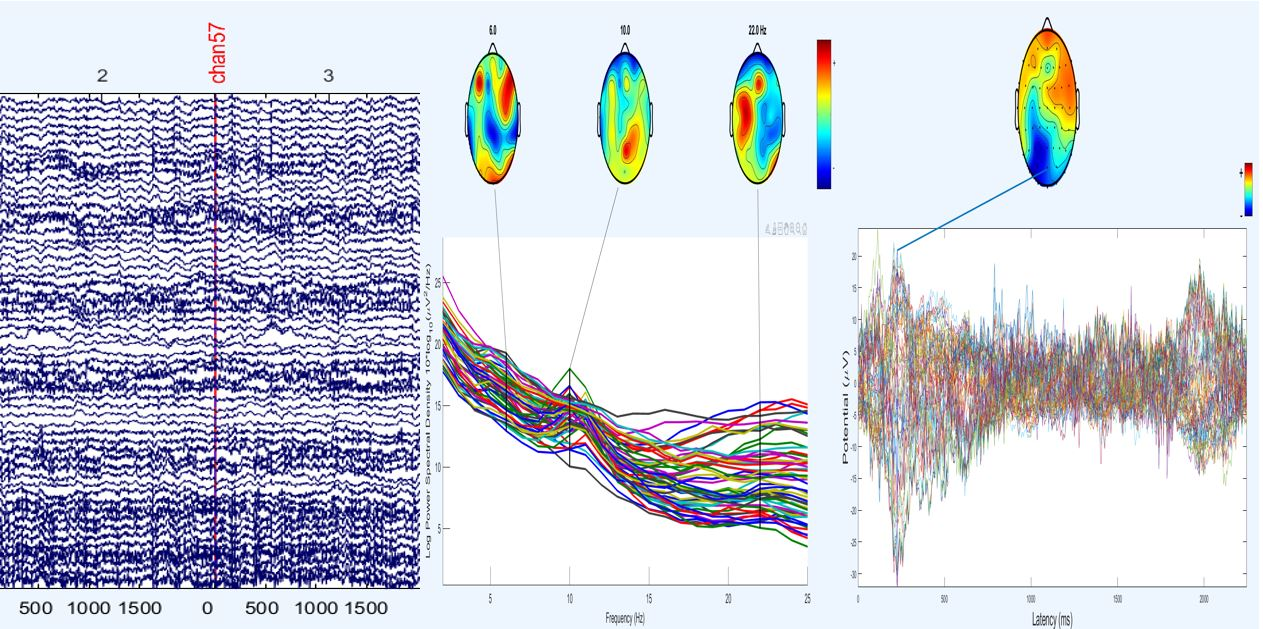
\includegraphics[keepaspectratio, scale=0.4]{pic/brain.JPG}
            \end{center}
        \end{figure}
    \end{itemize}
\end{frame}


\begin{frame}{High Dimensional Data}
    \begin{itemize}
        \item High-Dimensions  = Lots of	Features
        \item High Resolution Images (Millions of Pixels)
        \begin{figure}[htpb]
            \begin{center}
                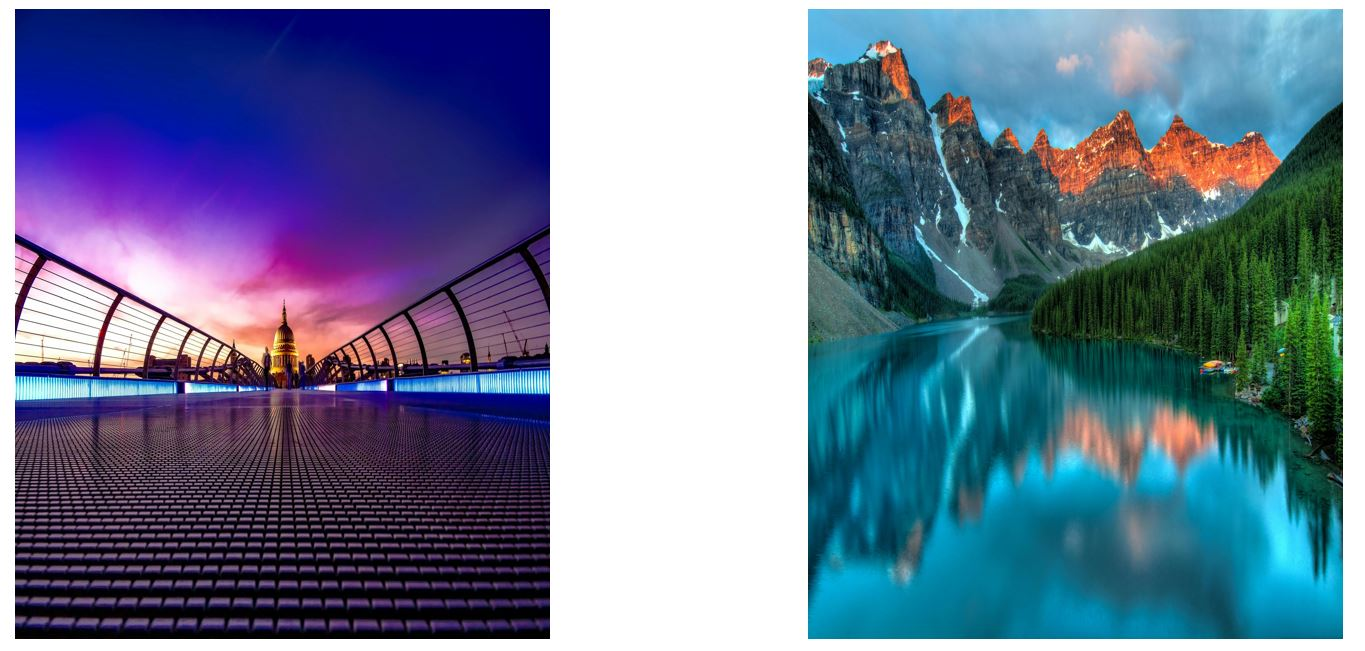
\includegraphics[keepaspectratio, scale=0.4]{pic/highRes.JPG}
            \end{center}
        \end{figure}
    \end{itemize}
\end{frame}


\begin{frame}{Dimensionality Reduction }
    \begin{itemize}
        \item \textbf{Feature Selection}
            \begin{itemize}
                \item Select a subset of a given feature set
            \end{itemize}

         \item \textbf{Feature Extraction}
            \begin{itemize}
                \item A linear or non-linear transform on the original feature space
            \end{itemize}
            \begin{figure}[htpb]
                \begin{center}
                    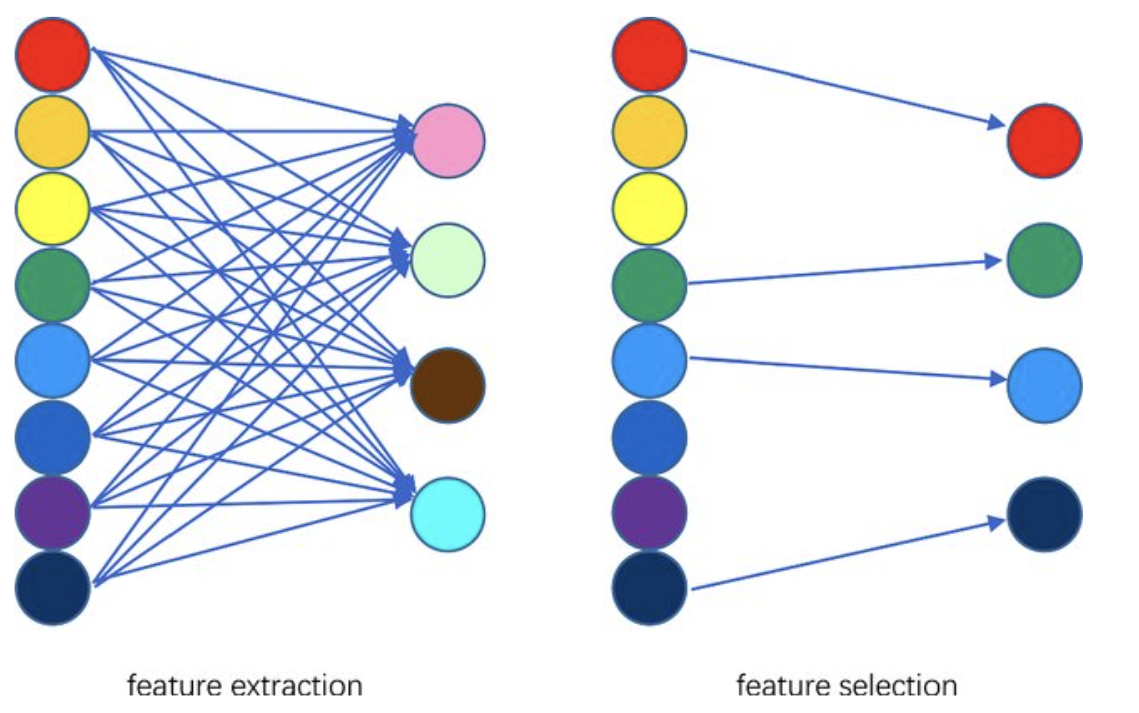
\includegraphics[keepaspectratio, scale=0.25]{pic/FS-FE.png}
                \end{center}
            \end{figure}
    \end{itemize}
\end{frame}


\begin{frame}{Dimensionality Reduction Benefits}
    \begin{itemize}
        \item \textbf{Visualization}
            \begin{itemize}
                \item Project high dimensional data into 2D or 3D
            \end{itemize}
        \item \textbf{More efficient use of resources}
            \begin{itemize}
                \item Time, Memory, CPU
            \end{itemize}
        \item \textbf{Statistical}
            \begin{itemize}
                \item Fewer dimensions leads to better generalization
            \end{itemize}
        \item \textbf{Removing Noise}
        \item \textbf{Pre-Process}
            \begin{itemize}
                \item Improve accuracy by reducing features
                \item As a Preprocessing step to reduce dimensions for supervised learning tasks
                \item Helps avoiding overfitting
            \end{itemize}
    \end{itemize}
\end{frame}

\section{Principal Component Analysis (PCA)}

\begin{frame}{Definition}
    \begin{itemize}
        \item \textbf{Goal} is reducing the dimensionality of the data while preserving important aspects of the data
        \item \textbf{Principal Components (PCs)} are orthogonal vectors that are ordered by the fraction of the total information (variation) in the corresponding directions
        \begin{itemize}
            \item Find the directions at which data approximately lie
        \end{itemize}
    \end{itemize}
\end{frame}

\begin{frame}{Definition}
    Orthogonal projection of the data onto a \textbf{lower-dimensional} linear space that:
    \begin{itemize}
        \item Maximizes variance of projected data
        \item Minimizes sum of squared distances to the line
    \end{itemize}
    \begin{figure}[htpb]
        \begin{center}
            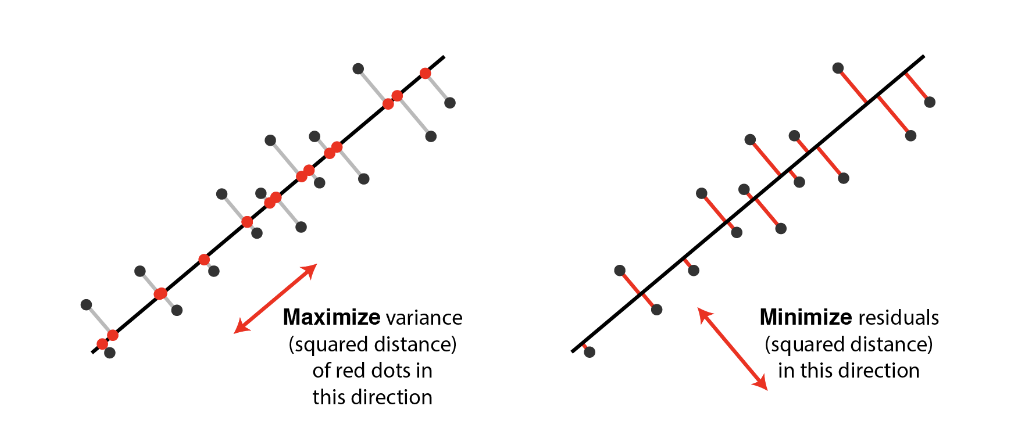
\includegraphics[keepaspectratio, scale=0.4]{pic/pca.png}
        \end{center}
    \end{figure}
\end{frame}

\begin{frame}{Definition}
    \begin{itemize}
        \item Minimizing sum of square distances to the line is \textbf{equivalent} to maximizing the sum of squares of the projections on that line.
    \end{itemize}
    \begin{figure}[htpb]
        \begin{center}
            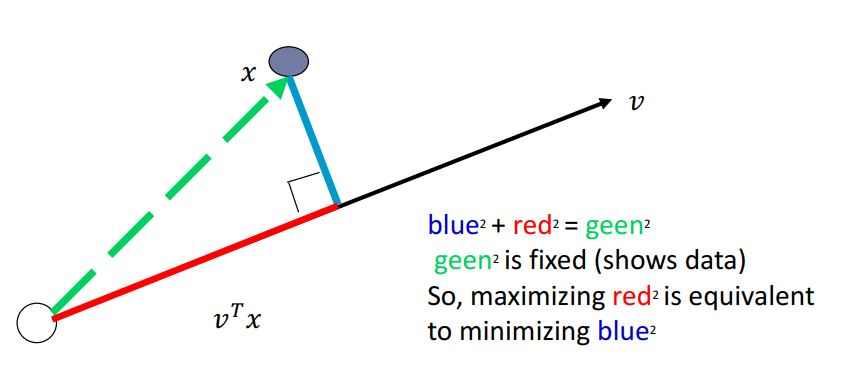
\includegraphics[keepaspectratio, scale=0.55]{pic/var_vs_rec.JPG}
        \end{center}
    \end{figure}
\end{frame}

\begin{frame}{Idea}
    \begin{itemize}
        \item Given data points in a d-dimensional space, project them into a lower dimensional space while preserving as much information as possible,
        \begin{itemize}
            \item Find best planar approximation of 3D data
            \item Find best 12-D approximation of 104-D data
        \end{itemize}
        \item In particular, choose projection that minimizes squared error in reconstructing the original data
    \end{itemize}
\end{frame}

\begin{frame}{Idea}
    \begin{itemize}
        \item 2D Gaussian dataset
         \begin{figure}[htpb]
            \begin{center}
                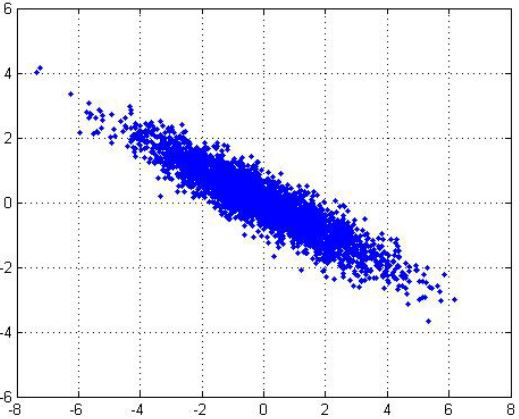
\includegraphics[keepaspectratio, scale=0.6]{pic/pcaData.JPG}
            \end{center}
        \end{figure}
    \end{itemize}
\end{frame}

\begin{frame}{Idea}
    \begin{itemize}
        \item 2D Gaussian dataset
        \item First PCA axis
         \begin{figure}[htpb]
            \begin{center}
                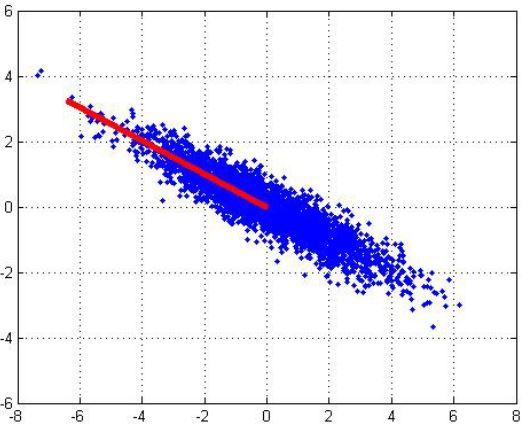
\includegraphics[keepaspectratio, scale=0.6]{pic/pcaData1.JPG}
            \end{center}
        \end{figure}
    \end{itemize}
\end{frame}

\begin{frame}{Idea}
    \begin{itemize}
        \item 2D Gaussian dataset
        \item First and second PCA axes
         \begin{figure}[htpb]
            \begin{center}
                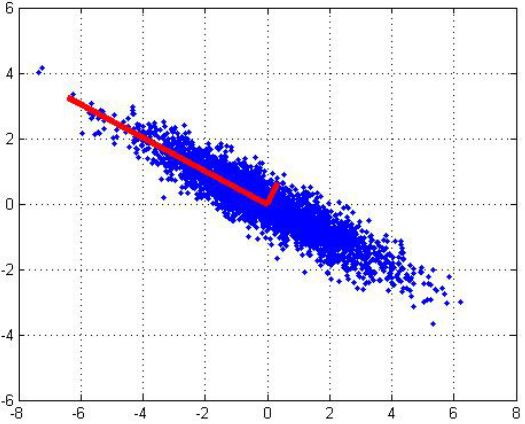
\includegraphics[keepaspectratio, scale=0.6]{pic/pcaData2.JPG}
            \end{center}
        \end{figure}
    \end{itemize}
\end{frame}

\begin{frame}{Random vs Principal Projection}
    \begin{itemize}
        \item Random direction vs. principal component
        \begin{figure}[htpb]
            \begin{center}
                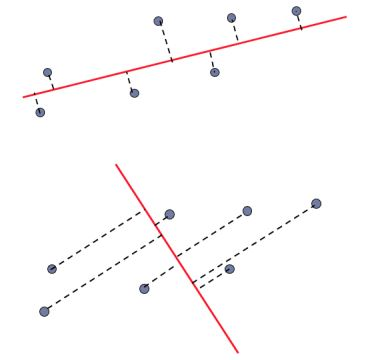
\includegraphics[keepaspectratio, scale=0.8]{pic/pcaVSrandom.JPG}
            \end{center}
        \end{figure}
    \end{itemize}
\end{frame}


\begin{frame}{Pre-processing}
    \begin{itemize}
        \item \textbf{Center the data}
            \begin{itemize}
                \item \textbf{Zero}ing out the \textbf{mean} of each feature\\
            \end{itemize}
            
        \item \textbf{Scaling to normalize each feature to have variance 1}
            \begin{itemize}
                \item An arbitrary step (May affect the final result!)
                \item It helps when unit of measurements of features are different and some features may be ignored without normalization
            \end{itemize}
    \end{itemize}
\end{frame}


\begin{frame}{Pre-processing}
    \begin{itemize}
        \item Scaling to normalize each feature may affect the final result!!
        \begin{figure}[htpb]
            \begin{center}
                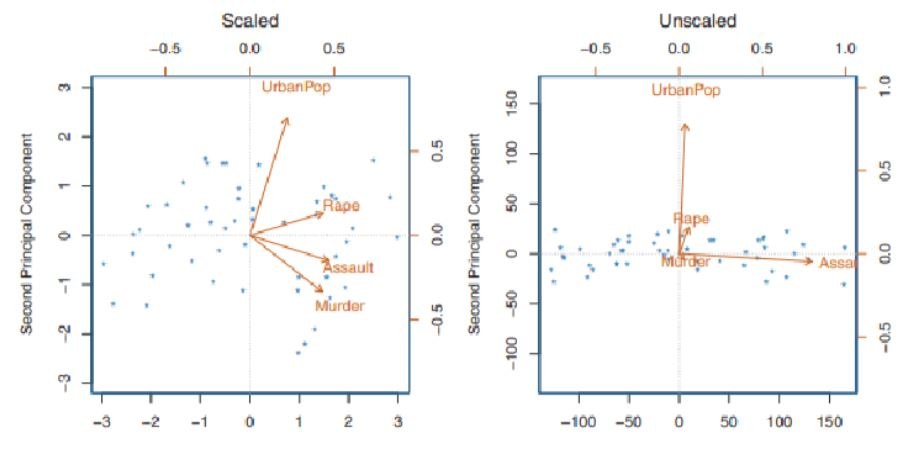
\includegraphics[keepaspectratio, scale=0.6]{pic/pcaScaling.JPG}
            \end{center}
        \end{figure}
    \end{itemize}
\end{frame}


\begin{frame}{Algorithms}
    \begin{itemize}
        \item Algorithm 1: sequential
        \item Algorithm 2: sample covariance matrix
    \end{itemize}
\end{frame}

\subsection{Sequential Algorithm}

\begin{frame}{Sequential Algorithm}
    \begin{itemize}
        \item First view
        \begin{itemize}
            \item Find directions with the maximum variations 
        \end{itemize}
        $$
        \max_{v_1} \frac{1}{N} \sum_{n=1}^{N} (v_1^T x_n)^2 = \frac{1}{N} \sum_{n=1}^{N} v_1^T (x_n x_n^T) v_1 = v_1^T \left( \frac{1}{N} \sum_{n=1}^{N}(x_n x_n^T) \right) v_1 = v_1^T S {v_1}
        $$
        $$ \text{s.t. } v_1^{T}{v_1}  = 1$$
        \begin{figure}[htpb]
            \begin{center}
                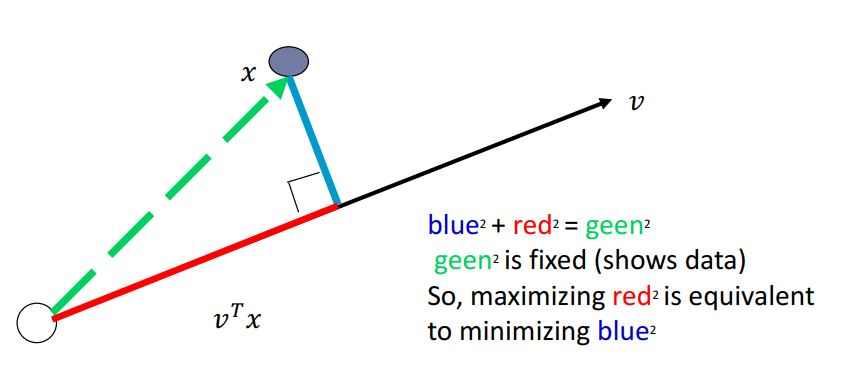
\includegraphics[keepaspectratio, scale=0.6]{pic/var_vs_rec.JPG}
            \end{center}
        \end{figure}
    \end{itemize}
\end{frame}

\begin{frame}{Sequential Algorithm}
    \begin{itemize}
        \item First view
        \item why $v_1^{T}{v_1} = 1$?
        \item Eigenvector with maximum eigenvalue maximizes the objective
        \begin{itemize}
            \item  Using Lagrangian multiplier technique
        \end{itemize}
        $$ L(v_1, \lambda) = v_1^T S v_1 + \lambda (1 - v_1^T v_1) $$
        $$ \frac{\partial L}{\partial v_1} = 0 \Rightarrow 2Sv_1 - 2\lambda v_1 = 0
 $$
        $$ \Rightarrow Sv_1 = \lambda v_1 $$
        
    \end{itemize}
\end{frame}

\begin{frame}{Sequential Algorithm}
    \begin{itemize}
        \item First view
        \item To find $v_2$, we maximize the variance of the projection in the residual subspace
$$
v_2 = max_{v_2} \left( \frac{1}{N} \sum_{i=1}^{N} \left( x_i - v_1^T x_i \right)^2 \right)
$$
$$ \text{s.t. } v_2^{T}{v_2}  = 1$$
          \item To find $v_k$, we maximize the variance of the projection in the residual subspace
$$
v_k = max_{v_k} \left( \frac{1}{N} \sum_{i=1}^{N} \left( x_i - \sum_{j=1}^{k-1} W_j^T x_i \right)^2 \right)
$$      
$$ \text{s.t. } v_k^{T}{v_k}  = 1$$
    \end{itemize}
\end{frame}

\begin{frame}{Sequential Algorithm}
    \begin{itemize}
        \item Second view
        \begin{itemize}
            \item Find directions with the minimum reconstruction error 
        \end{itemize}
        $$
        \min_{v1} \sum_{n=1}^{N} \lVert x_n - (v_{1}^{T} x_n)v_{1} \rVert_2^{2}
        $$
        $$ \text{s.t. } v_1^{T}{v_1}  = 1$$
        \item Show this has an equal solution with the first view

        \begin{figure}[htpb]
            \begin{center}
                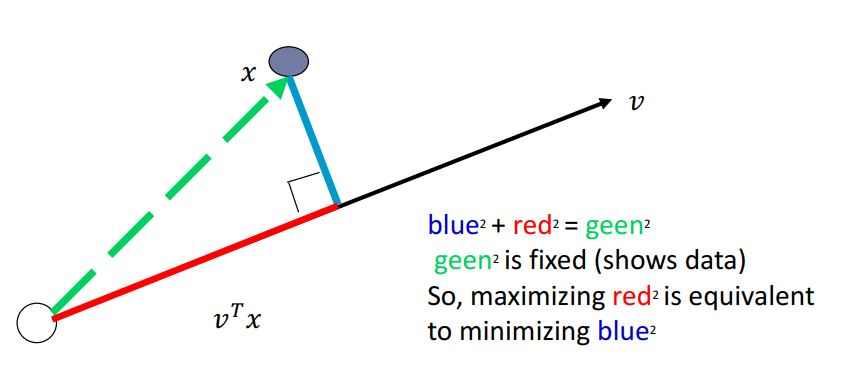
\includegraphics[keepaspectratio, scale=0.55]{pic/var_vs_rec.JPG}
            \end{center}
        \end{figure}

    \end{itemize}
\end{frame}


\begin{frame}{Sequential Algorithm}
    \begin{itemize}
       \item As we have $S v_j = \lambda_j v_j$,

    $$\Rightarrow \text{var}(v_j^T x) = v_j^T x x^{T} v_j =
       v_j^T S v_j =
       \lambda_j v_j^T v_j =
       \lambda_j$$.
    
    \item The variance along an eigenvector  $v_j \text{ equals the eigenvalue } \lambda_j. $
        
    \end{itemize}
\end{frame}


\begin{frame}{Sequential Algorithm}
    \begin{itemize}
       \item Eigenvalues: $\lambda_1 \geq \lambda_2 \geq \lambda_3 \geq ... $
        \begin{itemize}
            \item The first PC $v_1$ is the the eigenvector of the sample covariance matrix $S$ associated with the largest eigenvalue
            \item The 2nd PC $v_2$ is the the eigenvector of the sample covariance
matrix $S$ associated with the second largest eigenvalue
            \item And so on ...
        \end{itemize}
         \item To reduce the dimension of the data to k, we select eigenvectors with the top k eigenvalues
        
    \end{itemize}
\end{frame}


\subsection{Sample Covariance Matrix Algorithm}

\begin{frame}{Sample Covariance Matrix}
    \begin{itemize}
        \item Given data ${x_1, …, x_n}$, compute covariance matrix $\Sigma$
        $$\Sigma = \frac{1}{N} \sum_{i=1}^{N} (x_i - \bar{x})(x_i - \bar{x})^T \text{ where }  \bar{x} = \frac{1}{N} \sum_{i=1}^{N} x_i $$
        \item PCA basis vectors = the eigenvectors of $\Sigma$
        \item Larger eigenvalue $\rightarrow$ more important eigenvectors
    \end{itemize}
\end{frame}

% \begin{frame}{}
%     \begin{itemize}
%         \item Input: $N * d$ data matrix $X$ (each row contain a $d$ dimensional data point)
%         \begin{itemize}
%             \item $\bar{x} = \frac{1}{N} \sum_{i=1}^{N} x_i$
%             \item $\tilde{X} \leftarrow $ Mean value of data points is subtracted from rows of $X$
%             \item $S = \frac{1}{N}\tilde{X}^{T}\tilde{X} \text{(Covariance matrix)}$
%             \item Calculate eigenvalue and eigenvectors of $S$
%             \item Pick $K$ eigenvectors corresponding to the largest eigenvalues
% and put them in the columns of $A = [v_1, ... , v_k]$
%             \item $X' = XA$
%         \end{itemize}
%     \end{itemize}
% \end{frame}

\begin{frame}{Sample Covariance Matrix}
    \begin{algorithm}[H]
    \caption{Sample Covariance Matrix}\label{alg:Sample Covariance Matrix}
    \begin{algorithmic}[1]
         \State \textbf{Input:} $X \in \mathbb{R}^{N \times d}$ (data matrix with $N$ data points and $d$ dimensions)
        \State Compute the mean of each feature: 
        \LeftComment{$\bar{x} = \frac{1}{N} \sum_{i=1}^{N} x_i$}
        \State Subtract the mean from each data point (center the data): 
        \LeftComment{$\tilde{X} \leftarrow X - 1_N\bar{x}^{T}$}
        \State Compute the covariance matrix: 
        \LeftComment{$S = \frac{1}{N} \tilde{X}^{T} \tilde{X}$}

        \State Compute the eigenvalues and eigenvectors of $S$: 
        \LeftComment{$[\lambda_1, \lambda_2, \dots, \lambda_d],  [v_1, v_2, \dots, v_d] = \text{eig}(S)$}
        \State Select the top $K$ eigenvectors corresponding to the largest eigenvalues: 
        \LeftComment{$A \leftarrow [v_1, v_2, \dots, v_K]$}
        \State Transform the data into the new subspace:
        \LeftComment{$X' \leftarrow X \cdot A$}
        \State \textbf{Output:} $X' \in \mathbb{R}^{N \times K}$ (transformed data with reduced dimensions)
    \end{algorithmic}
    \end{algorithm}
\end{frame}


\begin{frame}{Sample Covariance Matrix}
    \begin{itemize}
        \item Eigen-vectors of symmetric matrices are orthogonal
        \item Covariance matrix is symmetric
        \begin{itemize}
            \item Principal component are orthonormal
        \end{itemize}
        \item  We have
        $$
        v_i^T v_j = 0, \quad \forall i \neq j 
        $$
        $$
        v_i^T v_i = 1, \quad \forall i
        $$
    \end{itemize}
\end{frame}

\section{Choose PCs}

\begin{frame}{How many PCs?}
    \begin{itemize}
        \item For $n$ original dimensions, sample covariance matrix is $n * n$, and has up to $n$ eigenvectors. So $n$ PCs
        \item Can ignore the components of lesser significance
        \begin{figure}[htpb]
            \begin{center}
                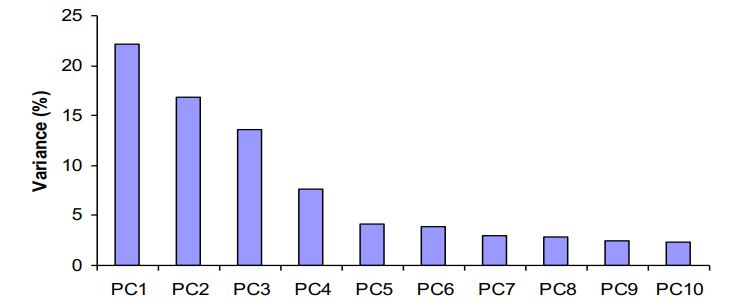
\includegraphics[keepaspectratio, scale=0.6]{pic/var.JPG}
            \end{center}
        \end{figure}
        \item You do lose some information, but if the eigenvalues are small, you don’t lose much
    \end{itemize}
\end{frame}

\begin{frame}{How many PCs?}
       $$\frac{\sum_{i=d-k+1}^{d} \lambda_i}{\sum_{i=1}^{d} \lambda_i}$$
       \begin{figure}[htpb]
            \begin{center}
                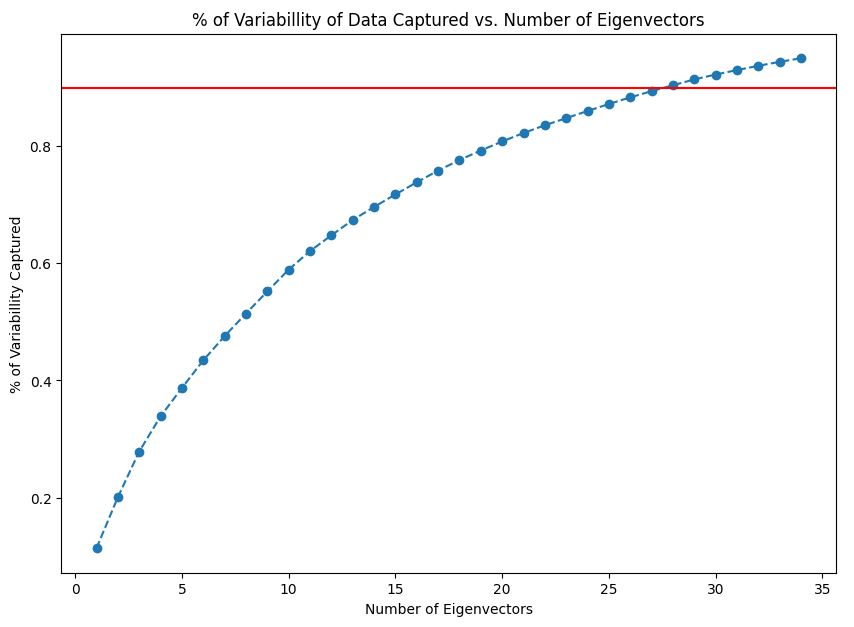
\includegraphics[keepaspectratio, scale=0.4]{pic/PCA_var.JPG}
            \end{center}
        \end{figure}
\end{frame}

\section{Applications}

\begin{frame}{Image Compression}
       \begin{itemize}
           \item Divide the original 372x492 image into patches
\begin{itemize}
    \item Each patch is an instance that contains 12x12 pixels on a grid
\end{itemize}
            \item Consider each as a 144-D vector
       \end{itemize}
        \begin{figure}[htpb]
            \begin{center}
                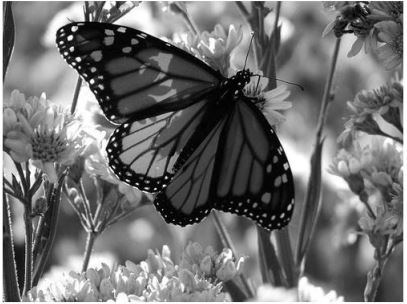
\includegraphics[width=8cm, height=5cm]{pic/original.JPG}
            \end{center}
        \end{figure}
\end{frame}

\begin{frame}{Image Compression}
       \begin{itemize}
           \item 144D $\Rightarrow$ 60D
       \end{itemize}
        \begin{figure}[htpb]
            \begin{center}
                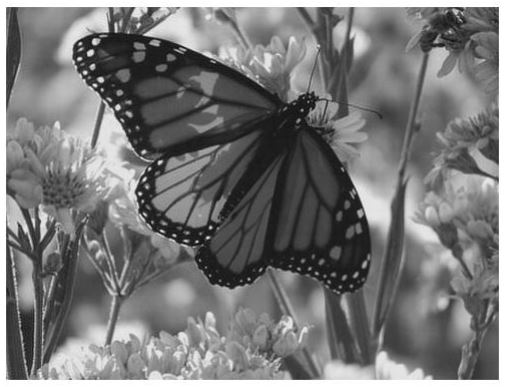
\includegraphics[width=8cm, height=5cm]{pic/60d.JPG}
            \end{center}
        \end{figure}
\end{frame}

\begin{frame}{Image Compression}
       \begin{itemize}
           \item 144D $\Rightarrow$ 16D
       \end{itemize}
        \begin{figure}[htpb]
            \begin{center}
                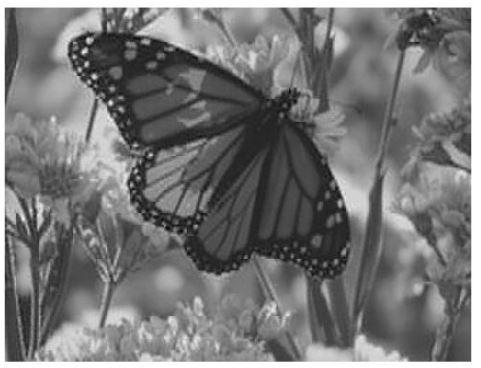
\includegraphics[width=8cm, height=5cm]{pic/16d.JPG}
            \end{center}
        \end{figure}
\end{frame}


\begin{frame}{Image Compression}
       \begin{itemize}
           \item 16 most important eigenvectors
       \end{itemize}
        \begin{figure}[htpb]
            \begin{center}
                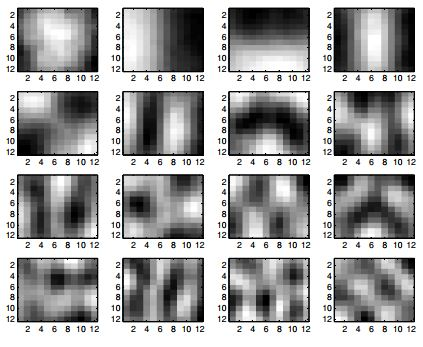
\includegraphics[width=8cm, height=5cm]{pic/16_most.JPG}
            \end{center}
        \end{figure}
\end{frame}


\begin{frame}{Image Compression}
       \begin{itemize}
           \item 144D $\Rightarrow$ 3D
       \end{itemize}
        \begin{figure}[htpb]
            \begin{center}
                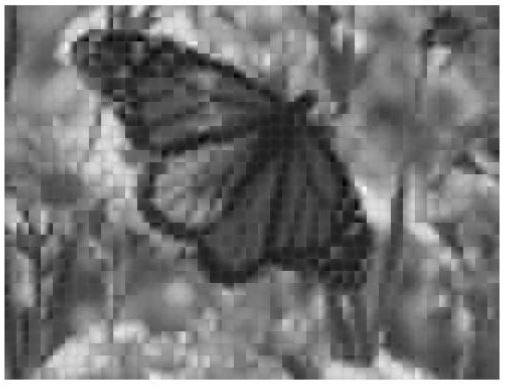
\includegraphics[width=8cm, height=5cm]{pic/3d.JPG}
            \end{center}
        \end{figure}
\end{frame}


\begin{frame}{Image Compression}
       \begin{itemize}
           \item 3 most important eigenvectors
       \end{itemize}
        \begin{figure}[htpb]
            \begin{center}
                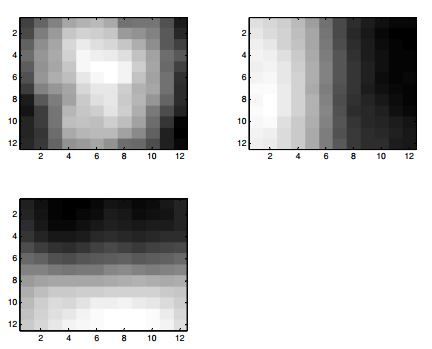
\includegraphics[width=8cm, height=5cm]{pic/3_most.JPG}
            \end{center}
        \end{figure}
\end{frame}


\begin{frame}{Image Compression}
       \begin{itemize}
           \item L2 error and PCA dim
       \end{itemize}
        \begin{figure}[htpb]
            \begin{center}
                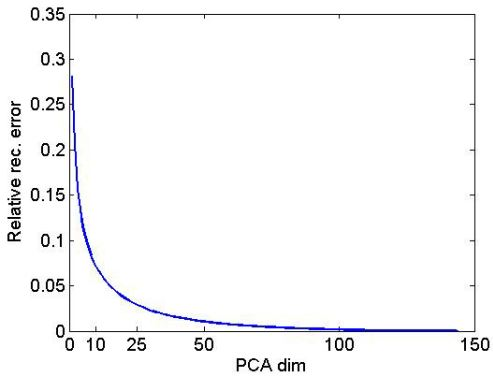
\includegraphics[width=8cm, height=5cm]{pic/error.JPG}
            \end{center}
        \end{figure}
\end{frame}

\section{Shortcomings}

\begin{frame}{Class Labels}
    \begin{itemize}
        \item PCA doesn’t know about class labels!
        \begin{figure}[htpb]
            \begin{center}
                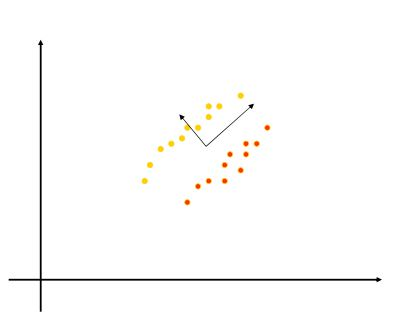
\includegraphics[width=8cm, height=5cm]{pic/labels.JPG}
            \end{center}
        \end{figure}
    \end{itemize}
\end{frame}


\begin{frame}{Non-Linear}
    \begin{itemize}
        \item PCA cannot capture Non-Linear structure!
        \begin{figure}[htpb]
            \begin{center}
                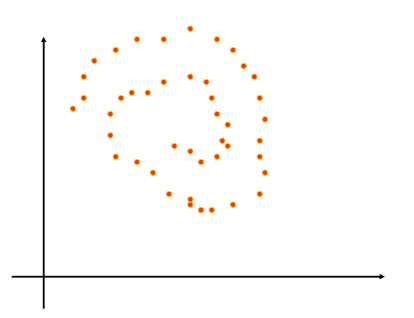
\includegraphics[width=8cm, height=5cm]{pic/nolinear.JPG}
            \end{center}
        \end{figure}
    \end{itemize}
\end{frame}

\section{Conclusion}

\begin{frame}{Conclusion}
    \begin{itemize}
        \item PCA 
        \begin{itemize}
            \item finds orthonormal basis for data
            \item Sorts dimensions in order of “importance”
            \item Discard low significance dimensions
        \end{itemize}
        \item Applications
        \begin{itemize}
            \item Get compact description
            \item Remove noise
            \item Improve classification (hopefully)
            \item More efficient use of resources
            \item Statistical
        \end{itemize}
        \item Not magic
        \begin{itemize}
            \item  Doesn’t know class labels
            \item Can only capture linear variations
        \end{itemize}
        \item One of many tricks to reduce dimensionality!
    \end{itemize}
\end{frame}

\section{References}

\begin{frame}{References}
    \begin{itemize}
        \item Advanced Introduction to Machine Learning, CMU-10715, Barnabás Póczos
        \item 10-701 Introduction to Machine Learning, CMU, Matt Gormley	
        \item 10-301/10-601 Introduction to Machine Learning, CMU, Matt	Gormley	
        \item CE-477: Machine Learning - CS-828: Theory of Machine Learning, Sharif University of Technology, Fatemeh Seyyedsalehi
    \end{itemize}
\end{frame}

\end{document}